\documentclass[onlymath]{beamer}
% \documentclass[onlymath,handout]{beamer}

% Macros used by all lectures, but not necessarily by excercises

%%% General setup and dependencies:

% \usetheme[ddcfooter,nosectionnum]{tud}
\usetheme[nosectionnum,pagenum,noheader]{tud}
% \usetheme[nosectionnum,pagenum]{tud}

% Increase body font size to a sane level:
\let\origframetitle\frametitle
% \renewcommand{\frametitle}[1]{\origframetitle{#1}\normalsize}
\renewcommand{\frametitle}[1]{\origframetitle{#1}\fontsize{10pt}{13.2}\selectfont}
\setbeamerfont{itemize/enumerate subbody}{size=\small} % tud defaults to scriptsize!
\setbeamerfont{itemize/enumerate subsubbody}{size=\small}
% \setbeamerfont{normal text}{size=\small}
% \setbeamerfont{itemize body}{size=\small}

\renewcommand{\emph}[1]{\textbf{#1}}

\def\arraystretch{1.3}% Make tables even less cramped vertically

\usepackage[ngerman]{babel}
\usepackage[utf8]{inputenc}
\usepackage[T1]{fontenc}

%\usepackage{graphicx}
\usepackage[export]{adjustbox} % loads graphicx
\usepackage{import}
\usepackage{stmaryrd}
\usepackage[normalem]{ulem} % sout command
% \usepackage{times}
\usepackage{txfonts}

% \usepackage[perpage]{footmisc} % reset footnote counter on each page -- fails with beamer (footnotes gone)
\usepackage{perpage}  % reset footnote counter on each page
\MakePerPage{footnote}

\usepackage{tikz}
\usetikzlibrary{arrows,positioning}
% Inspired by http://www.texample.net/tikz/examples/hand-drawn-lines/
\usetikzlibrary{decorations.pathmorphing}
\pgfdeclaredecoration{penciline}{initial}{
    \state{initial}[width=+\pgfdecoratedinputsegmentremainingdistance,
    auto corner on length=1mm,]{
        \pgfpathcurveto%
        {% From
            \pgfqpoint{\pgfdecoratedinputsegmentremainingdistance}
                      {\pgfdecorationsegmentamplitude}
        }
        {%  Control 1
        \pgfmathrand
        \pgfpointadd{\pgfqpoint{\pgfdecoratedinputsegmentremainingdistance}{0pt}}
                    {\pgfqpoint{-\pgfdecorationsegmentaspect
                     \pgfdecoratedinputsegmentremainingdistance}%
                               {\pgfmathresult\pgfdecorationsegmentamplitude}
                    }
        }
        {%TO 
        \pgfpointadd{\pgfpointdecoratedinputsegmentlast}{\pgfpoint{1pt}{1pt}}
        }
    }
    \state{final}{}
}
\tikzset{handdrawn/.style={decorate,decoration=penciline}}
\tikzset{every shadow/.style={fill=none,shadow xshift=0pt,shadow yshift=0pt}}
% \tikzset{module/.append style={top color=\col,bottom color=\col}}

% Use to make Tikz attributes with Beamer overlays
% http://tex.stackexchange.com/a/6155
\tikzset{onslide/.code args={<#1>#2}{%
  \only<#1| handout:0>{\pgfkeysalso{#2}} 
}}
\tikzset{onslideprint/.code args={<#1>#2}{%
  \only<#1>{\pgfkeysalso{#2}} 
}}

%%% Title -- always set this first

\newcommand{\defineTitle}[3]{
	\newcommand{\lectureindex}{#1}
	\title{Formale Systeme}
	\subtitle{\href{\lectureurl}{#1. Vorlesung: #2}}
	\author{\href{http://korrekt.org/}{Markus Kr\"{o}tzsch}}
%	\author{\href{http://www.sebastian-rudolph.de}{Sebastian Rudolph} in Vertretung von \href{http://korrekt.org/}{Markus Kr\"{o}tzsch}}
	\date{#3}
	\datecity{TU Dresden}
% 	\institute{Computational Logic}
}

%%% Table of contents:

\RequirePackage{ifthen}

\newcommand{\highlight}[2]{%
	\ifthenelse{\equal{#1}{\lectureindex}}{\alert{#2}}{#2}%
}

\def\myspace{-0.7ex}
\newcommand{\printtoc}{
\begin{tabular}{r@{$\quad$}l}
\highlight{1}{1.} & \highlight{1}{Willkommen/Einleitung formale Sprachen}\\[\myspace]
\highlight{2}{2.} & \highlight{2}{Grammatiken und die Chomsky-Hierarchie}\\[\myspace]
\highlight{3}{3.} & \highlight{3}{Endliche Automaten}\\[\myspace]
\highlight{4}{4.} & \highlight{4}{Complexity of FO query answering}\\[\myspace]
\highlight{5}{5.} & \highlight{5}{Conjunctive queries}\\[\myspace]
\highlight{6}{6.} & \highlight{6}{Tree-like conjunctive queries}\\[\myspace]
\highlight{7}{7.} & \highlight{7}{Query optimisation}\\[\myspace]
\highlight{8}{8.} & \highlight{8}{Conjunctive Query Optimisation / First-Order~Expressiveness}\\[\myspace]
\highlight{9}{9.} & \highlight{9}{First-Order~Expressiveness / Introduction to Datalog}\\[\myspace]
\highlight{10}{10.} & \highlight{10}{Expressive Power and Complexity of Datalog}\\[\myspace]
\highlight{11}{11.} & \highlight{11}{Optimisation and Evaluation of Datalog}\\[\myspace]
\highlight{12}{12.} & \highlight{12}{Evaluation of Datalog (2)}\\[\myspace]
\highlight{13}{13.} & \highlight{13}{Graph Databases and Path Queries}\\[\myspace]
\highlight{14}{14.} & \highlight{14}{Outlook: database theory in practice}
\end{tabular}
}

\newcommand{\overviewslide}{%
\begin{frame}\frametitle{Overview}
\printtoc
\medskip

Siehe \href{\lectureurl}{course homepage [$\Rightarrow$ link]} for more information and materials
\end{frame}
}

%%% Colours:

\usepackage{xcolor,colortbl}
\definecolor{redhighlights}{HTML}{FFAA66}
\definecolor{lightblue}{HTML}{55AAFF}
\definecolor{lightred}{HTML}{FF5522}
\definecolor{lightpurple}{HTML}{DD77BB}
\definecolor{lightgreen}{HTML}{55FF55}
\definecolor{darkred}{HTML}{CC4411}
\definecolor{darkblue}{HTML}{176FC0}%{1133AA}
\definecolor{nightblue}{HTML}{2010A0}%{1133AA}
\definecolor{alert}{HTML}{176FC0}
\definecolor{darkgreen}{HTML}{36AB14}
\definecolor{strongyellow}{HTML}{FFE219}
\definecolor{devilscss}{HTML}{666666}

\newcommand{\redalert}[1]{\textcolor{darkred}{#1}}

%%% Style commands

\newcommand{\quoted}[1]{\texttt{"}{#1}\texttt{"}}
\newcommand{\squote}{\texttt{"}} % straight quote
\newcommand{\Sterm}[1]{\ensuremath{\mathtt{\textcolor{purple}{#1}}}}    % letters in alphabets
\newcommand{\Snterm}[1]{\textsf{\textcolor{darkblue}{#1}}} % nonterminal symbols
\newcommand{\Sntermsub}[2]{\Snterm{#1}_{\Snterm{#2}}} % nonterminal symbols
\newcommand{\Slang}[1]{\textbf{\textcolor{black}{#1}}}    % languages
\newcommand{\Slangsub}[2]{\Slang{#1}_{\Slang{#2}}}    % languages
% Code
\newcommand{\Scode}[1]{\textbf{#1}}    % reserved words in program listings, e.g., "if"
\newcommand{\Scodelit}[1]{\textcolor{purple}{#1}}    % literals in program listings, e.g., strings
\newcommand{\Scomment}[1]{\textcolor{gray}{#1}}    % comment in program listings

\newcommand{\epstrastar}{\mathrel{\mathord{\stackrel{\epsilon}{\to}}{}^*}} % transitive reflexive closure of epsilon transitions in an epslion-NFA

\newcommand{\narrowcentering}[1]{\mbox{}\hfill#1\hfill\mbox{}}

\newcommand{\defeq}{\mathrel{:=}}

\newcommand{\Smach}[1]{\ensuremath{\mathcal{#1}}}    % machines

%%% Slide layout commands:

\newcommand{\sectionSlide}[1]{
\frame{\begin{center}
\LARGE
#1
\end{center}}
}
\newcommand{\sectionSlideNoHandout}[1]{
\frame<handout:0>{\begin{center}
\LARGE
#1
\end{center}}
}

\newcommand{\mydualbox}[3]{%
 \begin{minipage}[t]{#1}
 \begin{beamerboxesrounded}[upper=block title,lower=block body,shadow=true]%
    {\centering\usebeamerfont*{block title}#2}%
    \raggedright%
    \usebeamerfont{block body}
%     \small
    #3%
  \end{beamerboxesrounded}
  \end{minipage}
}
% 
\newcommand{\myheaderbox}[2]{%
 \begin{minipage}[t]{#1}
 \begin{beamerboxesrounded}[upper=block title,lower=block title,shadow=true]%
    {\centering\usebeamerfont*{block title}\rule{0pt}{2.6ex} #2}%
  \end{beamerboxesrounded}
  \end{minipage}
}

\newcommand{\mycontentbox}[2]{%
 \begin{minipage}[t]{#1}%
 \begin{beamerboxesrounded}[upper=block body,lower=block body,shadow=true]%
    {\centering\usebeamerfont*{block body}\rule{0pt}{2.6ex}#2}%
  \end{beamerboxesrounded}
  \end{minipage}
}

\newcommand{\mylcontentbox}[2]{%
 \begin{minipage}[t]{#1}%
 \begin{beamerboxesrounded}[upper=block body,lower=block body,shadow=true]%
    {\flushleft\usebeamerfont*{block body}\rule{0pt}{2.6ex}#2}%
  \end{beamerboxesrounded}
  \end{minipage}
}

% label=180:{\rotatebox{90}{{\footnotesize\textcolor{darkgreen}{Beispiel}}}}
% \hspace{-8mm}\ghost{\raisebox{-7mm}{\rotatebox{90}{{\footnotesize\textcolor{darkgreen}{Beispiel}}}}}\hspace{8mm}
\newcommand{\examplebox}[1]{%
	\begin{tikzpicture}[decoration=penciline, decorate]
		\pgfmathsetseed{1235}
		\node (n1) [decorate,draw=darkgreen, fill=darkgreen!10,thick,align=left,text width=\linewidth, inner ysep=2mm, inner xsep=2mm] at (0,0) {#1};
% 		\node (n2) [align=left,text width=\linewidth,inner sep=0mm] at (n1.92) {{\footnotesize\raisebox{3mm}{\textcolor{darkgreen}{Beispiel}}}};
% 		\node (n2) [decorate,draw=darkgreen, fill=darkgreen!10,thick, align=left,text width=\linewidth,inner sep=2mm] at (n1.90) {{\footnotesize\raisebox{0mm}{\textcolor{darkgreen}{Beispiel}}}};
	\end{tikzpicture}%
}%

\newcommand{\codebox}[1]{%
	\begin{tikzpicture}[decoration=penciline, decorate]
		\pgfmathsetseed{1236}
		\node (n1) [decorate,draw=strongyellow, fill=strongyellow!10,thick,align=left,text width=\linewidth, inner ysep=2mm, inner xsep=2mm] at (0,0) {#1};
	\end{tikzpicture}%
}%

\newcommand{\defbox}[1]{%
	\begin{tikzpicture}[decoration=penciline, decorate]
		\pgfmathsetseed{1237}
		\node (n1) [decorate,draw=darkred, fill=darkred!10,thick,align=left,text width=\linewidth, inner ysep=2mm, inner xsep=2mm] at (0,0) {#1};
	\end{tikzpicture}%
}%

\newcommand{\theobox}[1]{%
	\begin{tikzpicture}[decoration=penciline, decorate]
		\pgfmathsetseed{1240}
		\node (n1) [decorate,draw=darkblue, fill=darkblue!10,thick,align=left,text width=\linewidth, inner ysep=2mm, inner xsep=2mm] at (0,0) {#1};
	\end{tikzpicture}%
}%

\newcommand{\anybox}[2]{%
	\begin{tikzpicture}[decoration=penciline, decorate]
		\pgfmathsetseed{1240}
		\node (n1) [decorate,draw=#1, fill=#1!10,thick,align=left,text width=\linewidth, inner ysep=2mm, inner xsep=2mm] at (0,0) {#2};
	\end{tikzpicture}%
}%


\newsavebox{\mybox}%
\newcommand{\doodlebox}[2]{%
\sbox{\mybox}{#2}%
	\begin{tikzpicture}[decoration=penciline, decorate]
		\pgfmathsetseed{1238}
		\node (n1) [decorate,draw=#1, fill=#1!10,thick,align=left,inner sep=1mm] at (0,0) {\usebox{\mybox}};
	\end{tikzpicture}%
}%

% Common notation

\usepackage{amsmath,amssymb,amsfonts}
\usepackage{xspace}

\newcommand{\lectureurl}{https://iccl.inf.tu-dresden.de/web/FS2016}

\DeclareMathAlphabet{\mathsc}{OT1}{cmr}{m}{sc} % Let's have \mathsc since the slide style has no working \textsc

% Dual of "phantom": make a text that is visible but intangible
\newcommand{\ghost}[1]{\raisebox{0pt}[0pt][0pt]{\makebox[0pt][l]{#1}}}

\newcommand{\tuple}[1]{\langle{#1}\rangle}

%%% Annotation %%%

\usepackage{color}
\newcommand{\todo}[1]{{\tiny\color{red}\textbf{TODO: #1}}}



%%% Old macros below; move when needed

\newcommand{\blank}{\text{\textvisiblespace}} % empty tape cell for TM

% table syntax
\newcommand{\dom}{\textbf{dom}}
\newcommand{\adom}{\textbf{adom}}
\newcommand{\dbconst}[1]{\texttt{"#1"}}
\newcommand{\pred}[1]{\textsf{#1}}
\newcommand{\foquery}[2]{#2[#1]}
\newcommand{\ground}[1]{\textsf{ground}(#1)}
% \newcommand{\foquery}[2]{\{#1\mid #2\}} %% Notation as used in Alice Book
% \newcommand{\foquery}[2]{\tuple{#1\mid #2}}

\newcommand{\quantor}{\mathord{\reflectbox{$\text{\sf{Q}}$}}} % the generic quantor

% logic syntax
\newcommand{\Inter}{\mathcal{I}} %used to denote an interpretation
\newcommand{\Jnter}{\mathcal{J}} %used to denote another interpretation
\newcommand{\Knter}{\mathcal{K}} %used to denote yet another interpretation
\newcommand{\Zuweisung}{\mathcal{Z}} %used to denote a variable assignment

% query languages
\newcommand{\qlang}[1]{{\sf #1}} % Font for query languages
\newcommand{\qmaps}[1]{\textbf{QM}({\sf #1})} % Set of query mappings for a query language

%%% Complexities %%%

\hyphenation{Exp-Time} % prevent "Ex-PTime" (see, e.g. Tobies'01, Glimm'07 ;-)
\hyphenation{NExp-Time} % better that than something else

% \newcommand{\complclass}[1]{{\sc #1}\xspace} % font for complexity classes
\newcommand{\complclass}[1]{\ensuremath{\mathsc{#1}}\xspace} % font for complexity classes

\newcommand{\ACzero}{\complclass{AC$_0$}}
\newcommand{\LogSpace}{\complclass{L}}
\newcommand{\NLogSpace}{\complclass{NL}}
\newcommand{\PTime}{\complclass{P}}
\newcommand{\NP}{\complclass{NP}}
\newcommand{\coNP}{\complclass{coNP}}
\newcommand{\PH}{\complclass{PH}}
\newcommand{\PSpace}{\complclass{PSpace}}
\newcommand{\NPSpace}{\complclass{NPSpace}}
\newcommand{\ExpTime}{\complclass{ExpTime}}
\newcommand{\NExpTime}{\complclass{NExpTime}}
\newcommand{\ExpSpace}{\complclass{ExpSpace}}
\newcommand{\TwoExpTime}{\complclass{2ExpTime}}
\newcommand{\NTwoExpTime}{\complclass{N2ExpTime}}
\newcommand{\ThreeExpTime}{\complclass{3ExpTime}}
\newcommand{\kExpTime}[1]{\complclass{#1ExpTime}}
\newcommand{\kExpSpace}[1]{\complclass{#1ExpSpace}}


\defineTitle{25}{NP-Vollständigkeit}{23. Januar 2017}

\begin{document}

\maketitle

\sectionSlideNoHandout{Rückblick}

\begin{frame}\frametitle{Kompexitätsklassen}

\redalert{Komplexitätsklassen} sind Mengen von Sprachen, die man (grob) einteilt entsprechend der Ressourcen,
die eine TM zur Entscheidung ihres Wortproblems benötigt.\bigskip

\begin{tabular}{ccc}
\alert{deterministisch} & & \alert{nichtdeterministisch} \\[1ex]
$\Scomplclass{P}=\Scomplclass{PTime}$ & \alert{polynomielle Zeit} & $\Scomplclass{NP}=\Scomplclass{NPTime}$\\
$\Scomplclass{Exp}=\Scomplclass{ExpTime}$ & \alert{exponentielle Zeit} & $\Scomplclass{NExp}=\Scomplclass{NExpTime}$\\[1ex]
$\Scomplclass{L}=\Scomplclass{LogSpace}$ & \alert{logarithmischer Speicher} & $\Scomplclass{NL}=\Scomplclass{NLogSpace}$\\
$\Scomplclass{PSpace}$ & \alert{polynomieller Speicher} & $\Scomplclass{NPSpace}$\\
\end{tabular}

\end{frame}


\begin{frame}\frametitle{Deterministisch vs. nichtdeterministisch}

%
Welche Beziehungen haben diese Klassen zu anderen?\pause
{\footnotesize
\begin{itemize}
\item Die Beziehungen zwischen nichtdeterministischen Klassen sind analog zu denen im deterministischen Fall:\\[1ex]
\narrowcentering{$\Scomplclass{NL}\subseteq \Scomplclass{NP}\subseteq \Scomplclass{NPSpace}\subseteq \Scomplclass{NExp}$}
\pause
\item Eine DTM kann als NTM aufgefasst werden, d.h. die nichtdeterministischen Klassen sind immer stärker:\\[1ex]
\narrowcentering{$\Scomplclass{L}\subseteq \Scomplclass{NL}\qquad \Scomplclass{P}\subseteq \Scomplclass{NP}\qquad \Scomplclass{PSpace}\subseteq \Scomplclass{NPSpace}\qquad \Scomplclass{Exp}\subseteq \Scomplclass{NExp}$}
\pause
\item Man kann NTMs mit DTMs simulieren, aber das ist oft mit exponentiellen Mehrkosten verbunden (Vorlesung 19).
\pause
\item Der berühmte \alert{Satz von Savitch} besagt, dass speicherbeschränkte NTMs durch DTMs mit nur quadratischen Mehrkosten simuliert werden können. Insbesondere gilt damit $\Scomplclass{PSpace}= \Scomplclass{NPSpace}$.
\end{itemize}}
% Insgesamt ergeben sich folgende Beziehungen:
Zusammenfassung der wichtigsten bekannten Beziehungen:
\theobox{
\[\Scomplclass{L}\subseteq\Scomplclass{NL}\subseteq \Scomplclass{P}\subseteq\Scomplclass{NP}\subseteq\Scomplclass{PSpace}= \Scomplclass{NPSpace}\subseteq \Scomplclass{Exp}\subseteq \Scomplclass{NExp}\]
\vspace{-2.5ex}
}

\end{frame}

\begin{frame}\frametitle{Die Grenzen unseres Wissens}

Wir wissen:

\theobox{
\[\Scomplclass{L}\subseteq\Scomplclass{NL}\subseteq \Scomplclass{P}\subseteq\Scomplclass{NP}\subseteq\Scomplclass{PSpace}= \Scomplclass{NPSpace}\subseteq \Scomplclass{Exp}\subseteq \Scomplclass{NExp}\]
\vspace{-2.5ex}
}

\begin{itemize}
\item Wir wissen nicht, ob irgendeines dieser $\subseteq$ sogar $\subsetneq$ ist.
\item Insbesondere wissen wir nicht, ob $\Scomplclass{P}\subsetneq\Scomplclass{NP}$ oder $\Scomplclass{P}=\Scomplclass{NP}$.
\item Wir wissen nicht einmal, ob $\Scomplclass{L}\subsetneq\Scomplclass{NP}$ oder $\Scomplclass{L}=\Scomplclass{NP}$.
\end{itemize}\pause
Es wird aber vermutet, dass alle  $\subseteq$ eigentlich $\subsetneq$ sind.
% 
Bekannt ist das aber nur bei exponentiell großen Ressourcenunterschieden:

\theobox{Es gilt:
\begin{itemize}
\item $\Scomplclass{NL}\subsetneq\Scomplclass{PSpace}$
\item $\Scomplclass{P}\subsetneq\Scomplclass{Exp}$
\item $\Scomplclass{NP}\subsetneq\Scomplclass{NExp}$
\end{itemize}}

\end{frame}


\sectionSlide{NP}

\begin{frame}\frametitle{NP-Probleme effizient lösen?}

Wir haben gesehen:
\[ \Slang{SAT}\in\Scomplclass{NP}\subseteq\Scomplclass{PSpace}\subseteq\Scomplclass{ExpTime}\]

\begin{itemize}
\item Dennoch haben alle unsere Algorithmen für $\Slang{SAT}$ bisher 
exponentielle Laufzeit.
\item $\Slang{SAT}\in\Scomplclass{NP}$ führt nicht direkt zu einer besseren Lösung, da real existierende Computer nicht wie NTMs arbeiten.
\item Andererseits spricht auch nichts dagegen, dass es einen schnelleren Algorithmus gibt.
\end{itemize}

\anybox{purple}{Kann man $\Slang{SAT}$ auch effizienter lösen?}
$\leadsto$ Dazu sollten wir erst einmal $\Scomplclass{NP}$ etwas besser verstehen

\end{frame}

\begin{frame}\frametitle{Lösungen prüfen}

\emph{Eine Interessante Eigenschaft von \Slang{SAT}:}
\begin{itemize}
\item Es scheint schwer, die Erfüllbarkeit einer Formel zu ermitteln (z.B. können wir exponentiell viele
	Wertzuweisungen durchsuchen).
\item Es ist einfach, Erfüllbarkeit einer Formel zu überprüfen, wenn ein Modell gegeben ist (dazu muss nur der Wahrheitswert der Formel berechnet werden).
\end{itemize}\pause

\emph{Ähnlich ist es bei Sudoku:}
\begin{itemize}
\item Es ist schwer, ein Sudoku korrekt auszufüllen.
\item Es ist einfach, zu prüfen, ob ein Sudoku korrekt ausgefüllt \ghost{wurde.}
\end{itemize}\pause

\anybox{purple}{
\emph{Gibt es noch mehr Probleme, die sich so verhalten?}
\begin{itemize}
\item Es ist schwer, eine Lösung zu finden.
\item Es ist einfach, eine gegebene Lösung zu prüfen.
\end{itemize}}

\end{frame}

\begin{frame}\frametitle{TMs die Lösungen überprüfen}

Wir wollen diese Idee formalisieren:

\defbox{Ein \redalert{polynomieller Verifikator} für eine Sprache $\Slang{L}\subseteq \Sigma^*$ ist eine
polynomiell-zeitbeschränkte, deterministische TM \Smach{M}, für die gilt:
\begin{itemize}
\item \Smach{M} akzeptiert nur Wörter der Form $w\# z$ mit:
	\begin{itemize}
	\item $w\in\Slang{L}$
	\item $z\in\Sigma^*$ ist ein \redalert{Zertifikat} polynomieller Länge\\(d.h. für \Smach{M} gibt es ein Polynom $p$ mit $|z|\leq p(|w|)$)
	\end{itemize}
\item Für jedes Wort $w\in\Slang{L}$ gibt es ein solches Wort $w\# z\in\Slang{L}(\Smach{M})$.
\end{itemize}
}

\emph{Intuition:}
\begin{itemize}
\item Das Zertifikat $z$ kodiert die Lösung des Problems $w$, die der Verifikator lediglich nachprüft.
\item Zertifikate sollten kurz sein, damit die Prüfung selbst nicht länger dauert als die Lösung des Problems.
\end{itemize}

Zertifikate werden auch \alert{Nachweis}, \alert{Beweis} oder \alert{Zeuge} genannt

\end{frame}

\begin{frame}\frametitle{Nachweis-polynomielle Sprachen}

\defbox{Eine Sprache $\Slang{L}$ ist \redalert{nachweis-polynomiell} wenn es für sie einen polynomiellen
Verifikator gibt.}\medskip\pause

\examplebox{Beispiel: \Slang{SAT} ist nachweis-polynomiell. Ein möglicher polynomiellen Verifikator für
\Slang{SAT} akzeptiert Wörter $F\#w$, wobei $F$ die Kodierung einer erfüllbaren Formel ist und $w$ eine Kodierung einer
Wertzuweisung, die $F$ erfüllt.}\medskip\pause

\examplebox{Beispiel: Jede Sprache $\Slang{L}\in\Scomplclass{P}$ ist nachweis-polynomiell. Als Verifikator
verwenden wir einfach einen polynomiell-zeitbeschränkten Entscheider für $\Slang{L}$. Das Zertifikat kann leer sein.}

\end{frame}

\begin{frame}\frametitle{Beispiel: Drei-Farben-Problem}

Das \redalert{Drei-Farben-Problem} besteht darin, die Knoten eines ungerichteten Graphen so mit den
drei Farben rot, grün und blau zu färben, dass keine zwei benachbarten Knoten die gleiche Farbe haben.
\medskip

\narrowcentering{
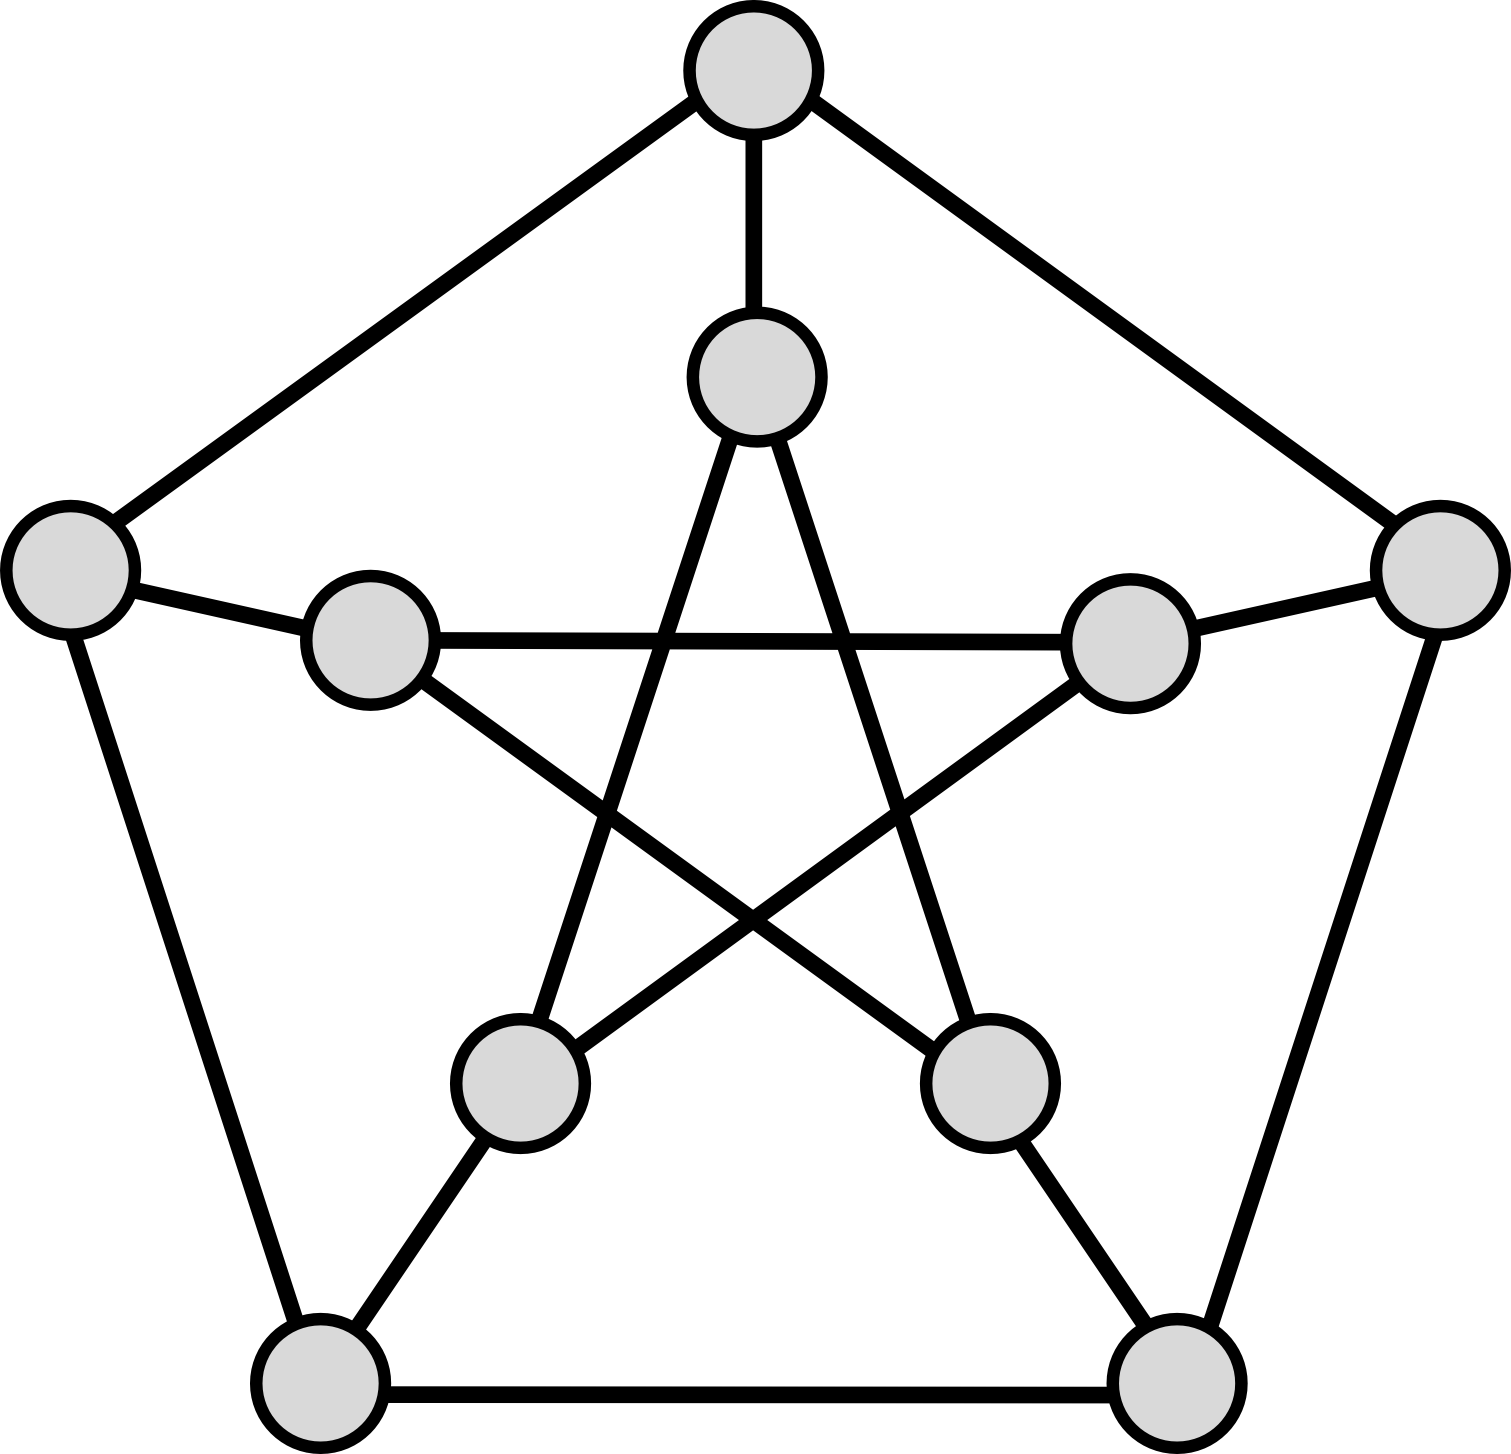
\includegraphics[width=3cm]{images/graph1}
\begin{minipage}[b]{3cm}
~\\\huge
\narrowcentering{$\Rightarrow$}\\[5mm]~
\end{minipage}
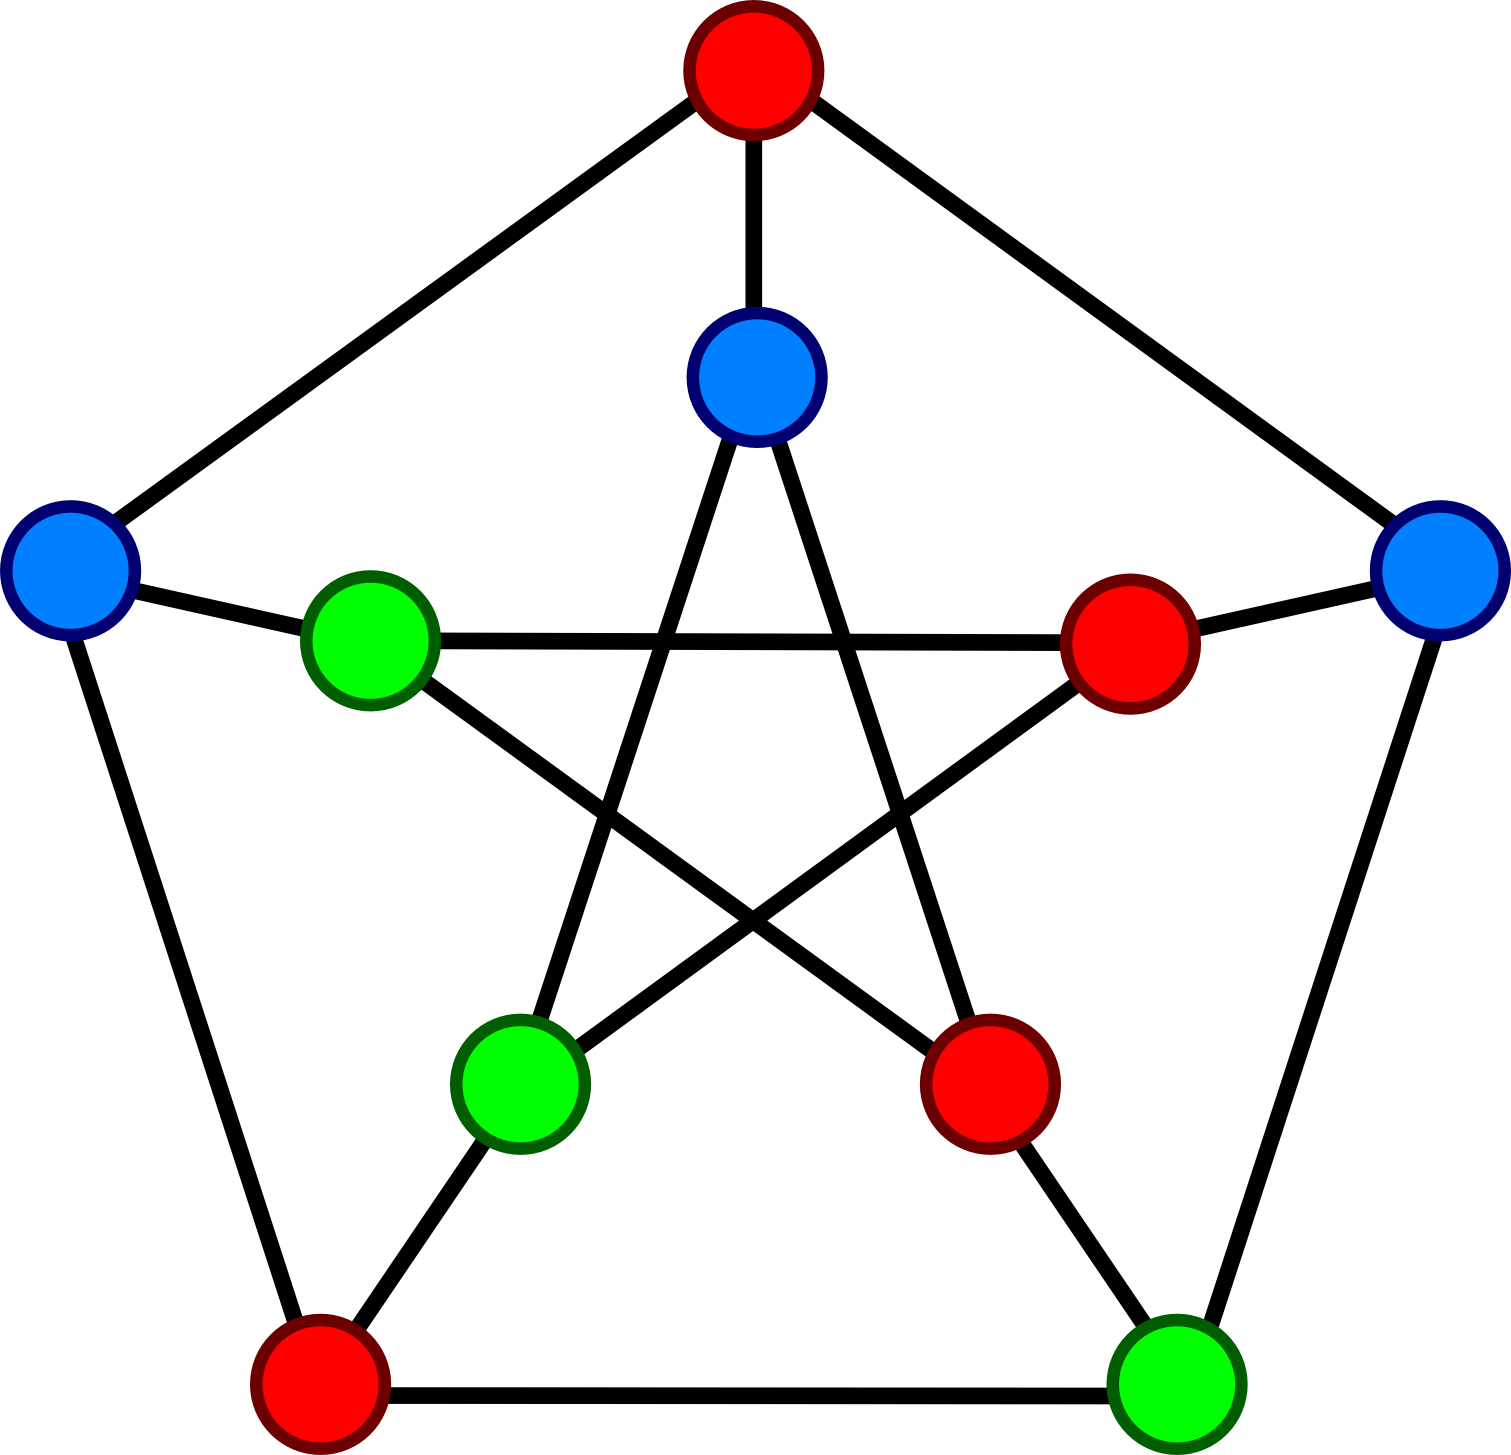
\includegraphics[width=3cm]{images/graph3}
}\pause

\medskip
Das Problem kann als Wortproblem aufgefasst werden, wenn man Graphen als Wörter kodiert (z.B. als Adjazenzliste oder als zeilenweise kodierte Adjazenzmatrix).
\medskip

\alert{Das Drei-Farben-Problem ist nachweis-polynomiell}\\ (Zertifikat: Farbzuweisung).

\end{frame}

\begin{frame}\frametitle{Beispiel: Faktorisierung}

\defbox{Die \redalert{Faktorisierung} einer natürlichen Zahl $n$ ist die Darstellung der 
Zahl als Produkt von natürlichen Zahlen $f_1\cdot f_2=n$.}\medskip

Folgende Sprache ist nachweis-polynomiell:\\[1ex]
\narrowcentering{$\Slang{COMPOSITE}=\{\textsf{bin}(n)\mid \text{es gibt }f_1,f_2>1 \text{ mit }n=f_1\cdot f_2\}$}\\[1ex]
(Zertifikat: Kodierung von $f_1$ und $f_2$)
\bigskip\pause

Überraschender Weise ist auch folgende Sprache nachweis-polynomiell:\\[1ex]
\narrowcentering{$\Slang{PRIMES}=\{\textsf{bin}(n)\mid \text{es gibt \redalert{keine} }f_1,f_2>1 \text{ mit }n=f_1\cdot f_2\}$}\\[1ex]
(Zertifikat: "`\href{https://en.wikipedia.org/wiki/Primality_certificate}{Primality certificate}"', bekannt seit 1975)
\bigskip\pause

\textcolor{devilscss}{(Seit 2002 wissen wir: $\textbf{PRIMES}\in\Scomplclass{P}$}\\
\textcolor{devilscss}{$\leadsto$ Primzahlentest nach Agrawal, Kayal und Saxena)}

\end{frame}

\begin{frame}[t]\frametitle{NP steht für "`nachweis-polynomiell"' (1)}

\theobox{Satz: Eine Sprache $\Slang{L}$ ist genau dann nachweis-polynomiell wenn $\Slang{L}\,{\in}\,\Scomplclass{NP}$.}\medskip\pause

\emph{Beweis:}
$(\Rightarrow)$ Sei $\Slang{L}$ nachweis-polynomiell mit Verifikator \Smach{V}. Wir erhalten eine polynomiell-zeitbeschränkte NTM \Smach{M} für $\Slang{L}$ wie folgt:\pause
\begin{itemize}
\item für eine Eingabe $w$ rät \Smach{M} nichtdeterministisch ein polynomielles Zertifikat $z$\\
(dabei muss \Smach{M} die Länge von $z$ selbst beschränken)
\item anschließend führt \Smach{M} die Berechnungen wie \Smach{V} aus um das geratene Zertifikat in polynomieller Zeit zu prüfen
\end{itemize}

\end{frame}

\begin{frame}[t]\frametitle{NP steht für "`nachweis-polynomiell"' (2)}

\theobox{Satz: Eine Sprache $\Slang{L}$ ist genau dann nachweis-polynomiell wenn $\Slang{L}\,{\in}\,\Scomplclass{NP}$.}\medskip

\emph{Beweis:}
$(\Leftarrow)$ Sei \Smach{M} eine polynomiell-zeitbeschränkte NTM für $\Slang{L}$. Wir erhalten einen polynomiellen Verifikator \Smach{V} für $\Slang{L}$ wie folgt.\pause
% 
\begin{itemize}
\item Für jedes Wort $w\in\Slang{L}$ gibt es einen akzeptierenden Lauf von \ghost{\Smach{M}.}
\item In jedem Schritt dieses Laufs wählt \Smach{M} nichtdeterministisch einen Übergang aus.
\item Der Lauf ist von polynomieller Länge, da \Smach{M} polynomiell-zeitbeschränkt ist.
\end{itemize}\pause
$\leadsto$ Die Liste der Übergänge kann als Zertifikat dienen
\medskip

\Smach{V} prüft, ob die durch $z$ gegebenen Entscheidungen für die Eingabe $w$ zu einem akzeptierenden Lauf von \Smach{M} führen.\qed 

\end{frame}

\begin{frame}\frametitle{\Scomplclass{NP} ist nicht symmetrisch}

Es ist leicht zu sehen:

\theobox{Satz: Die Klasse \Scomplclass{P} ist unter Komplement abgeschlossen.}

\emph{Beweis:} Wenn es für \Slang{L} eine polynomiell-zeitbeschränkte TM \Smach{M}
gibt, dann erhält man eine TM für $\overline{\Slang{L}}$ indem man akzeptierende
und nicht-akzeptierende Zustände von \Smach{M} vertauscht.\qed
\medskip\pause

Für \Scomplclass{NP} ist das nicht so einfach möglich. Wir haben das schon für NFAs beobachtet (eine spezielle Art von NTMs).${}^*$

\examplebox{Beispiele: Es scheint kein einfaches Zertifikat dafür zu geben, dass
eine Formel \alert{nicht} erfüllbar ist oder dass ein Graph \alert{keine} Dreifärbung zulässt.
}\pause

\defbox{Die Klasse aller Sprachen $\Slang{L}$, für die $\overline{\Slang{L}}\in\Scomplclass{NP}$ gilt, heißt $\Scomplclass{coNP}$.}

% Jede nichtdeterministische Klasse kann so komplementiert werden, z.B. $\Scomplclass{coNL}$ oder $\Scomplclass{coNExp}$.
\medskip

{\tiny ${}^*$ Grund: für ein akzeptiertes Wort kann es bei einer NTM akzeptierende \emph{und} verwerfende Läufe geben. Nach dem Austausch der Endzustände gäbe es dann aber immer noch akzeptierende Läufe.\\
}

\end{frame}

\sectionSlide{NP-Vollständigkeit}

\definecolor{myred}{rgb}{0.80, 0.20, 0.20}
\definecolor{mygreen}{rgb}{0.20, 0.80, 0.20}
\definecolor{myblue}{rgb}{0.20, 0.20, 0.80}
\newcommand{\ppred}[1]{\color{myred}{\text{r}_{#1}}\color{text}{}}
\newcommand{\pgreen}[1]{\color{mygreen}{\text{g}_{#1}}\color{text}{}}
\newcommand{\pblue}[1]{\color{myblue}{\text{b}_{#1}}\color{text}{}}

\begin{frame}\frametitle{Reduktionen}

Manche Probleme lassen sich auf andere zurückführen\pause
\bigskip

% \bigskip
% 
% \alert{Beispiel:}\\
Beispiel: Drei-Farben-Problem ist auf \Slang{SAT} reduzierbar.
\bigskip

\only<2>{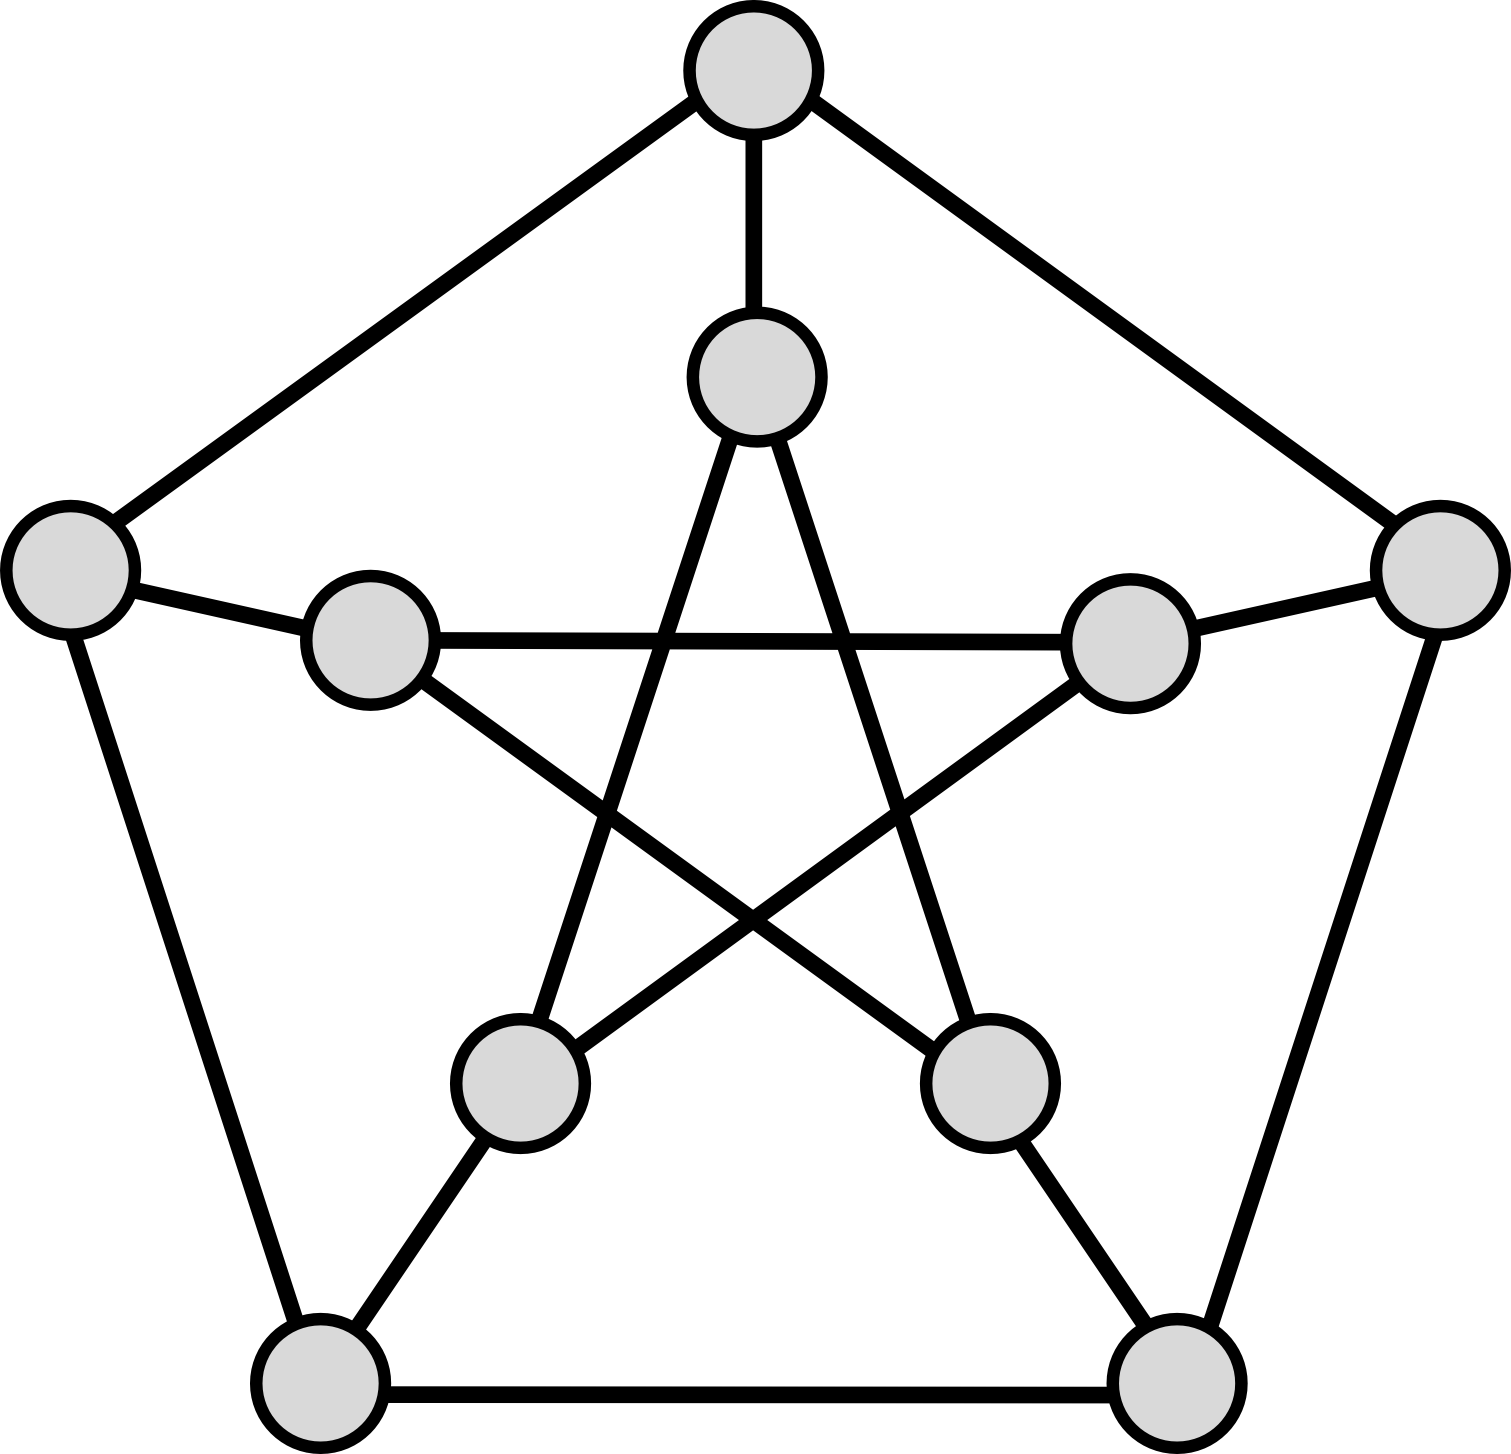
\includegraphics[width=2.5cm]{images/graph1}}%
\only<3-5>{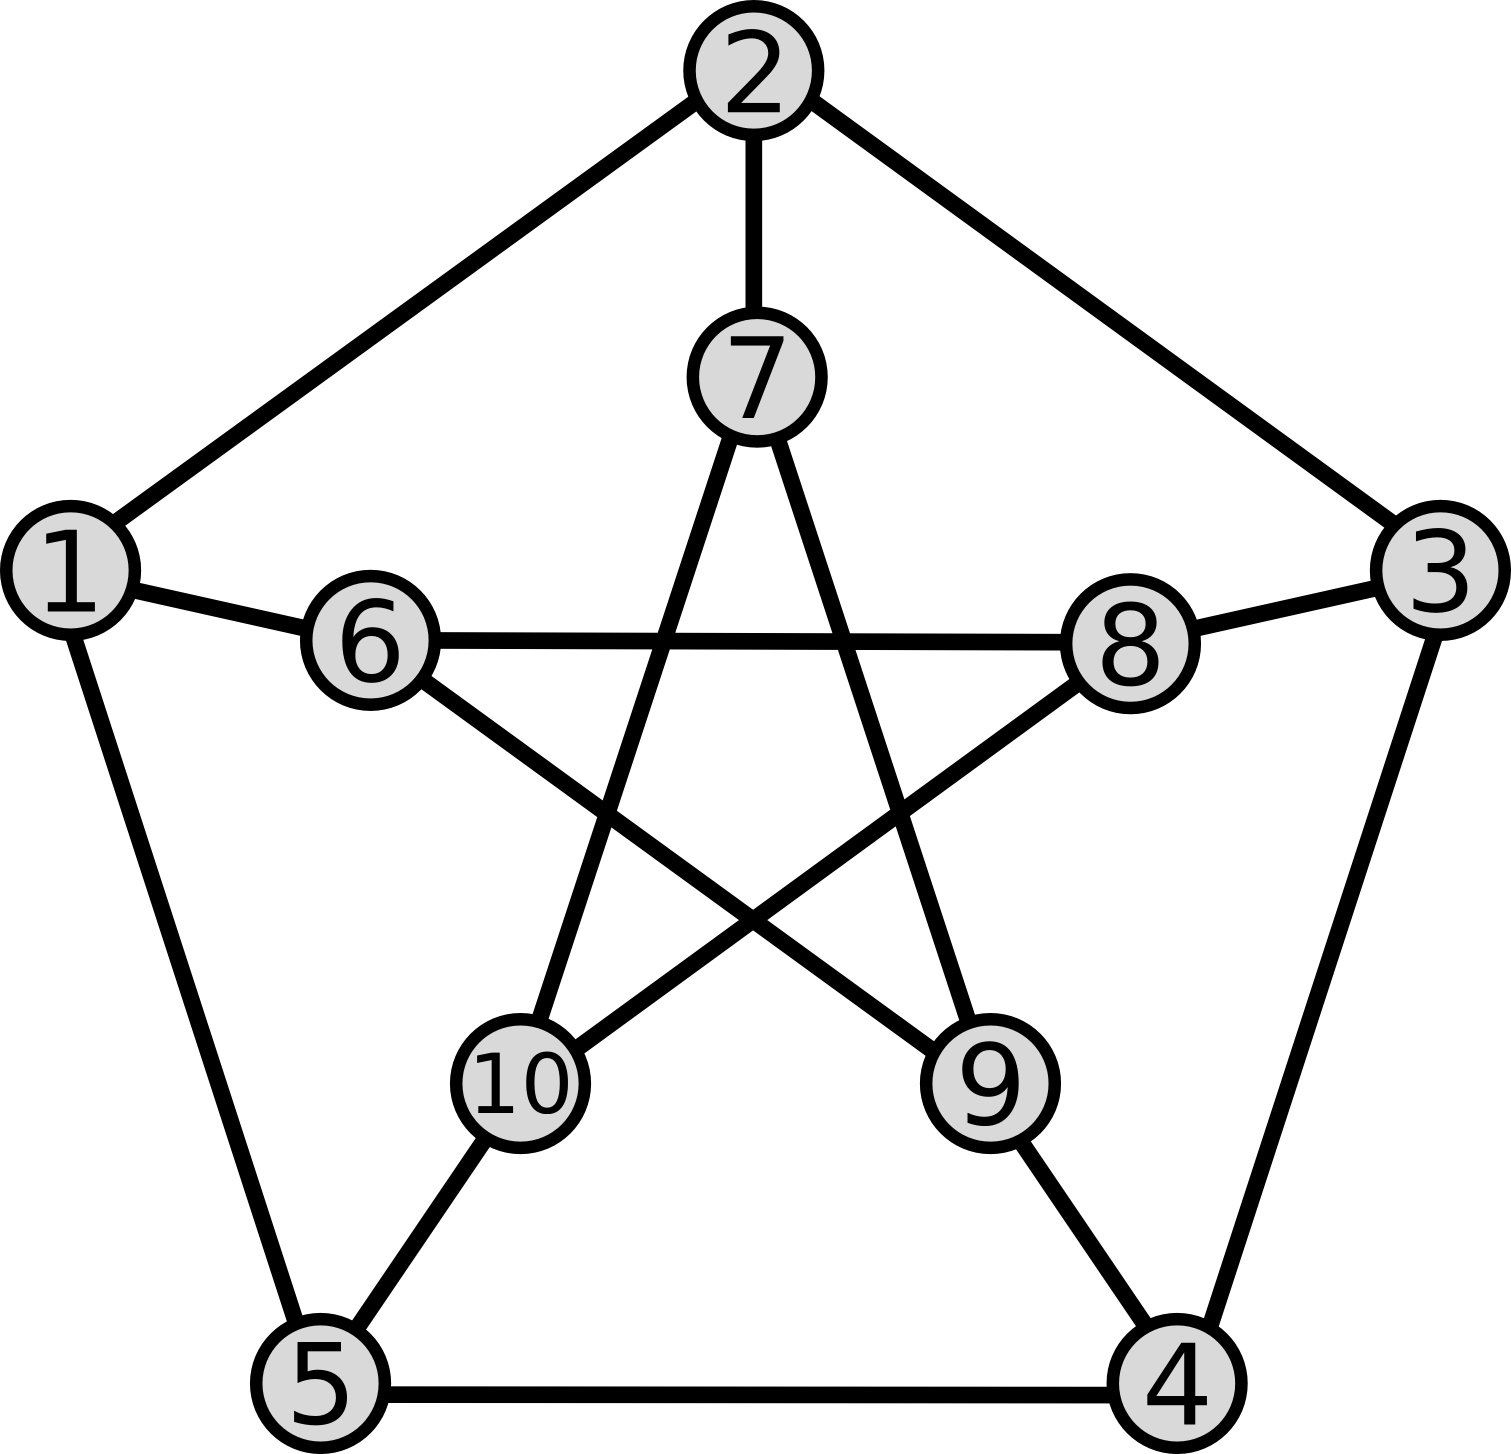
\includegraphics[width=2.5cm]{images/graph2}}%
\only<6->{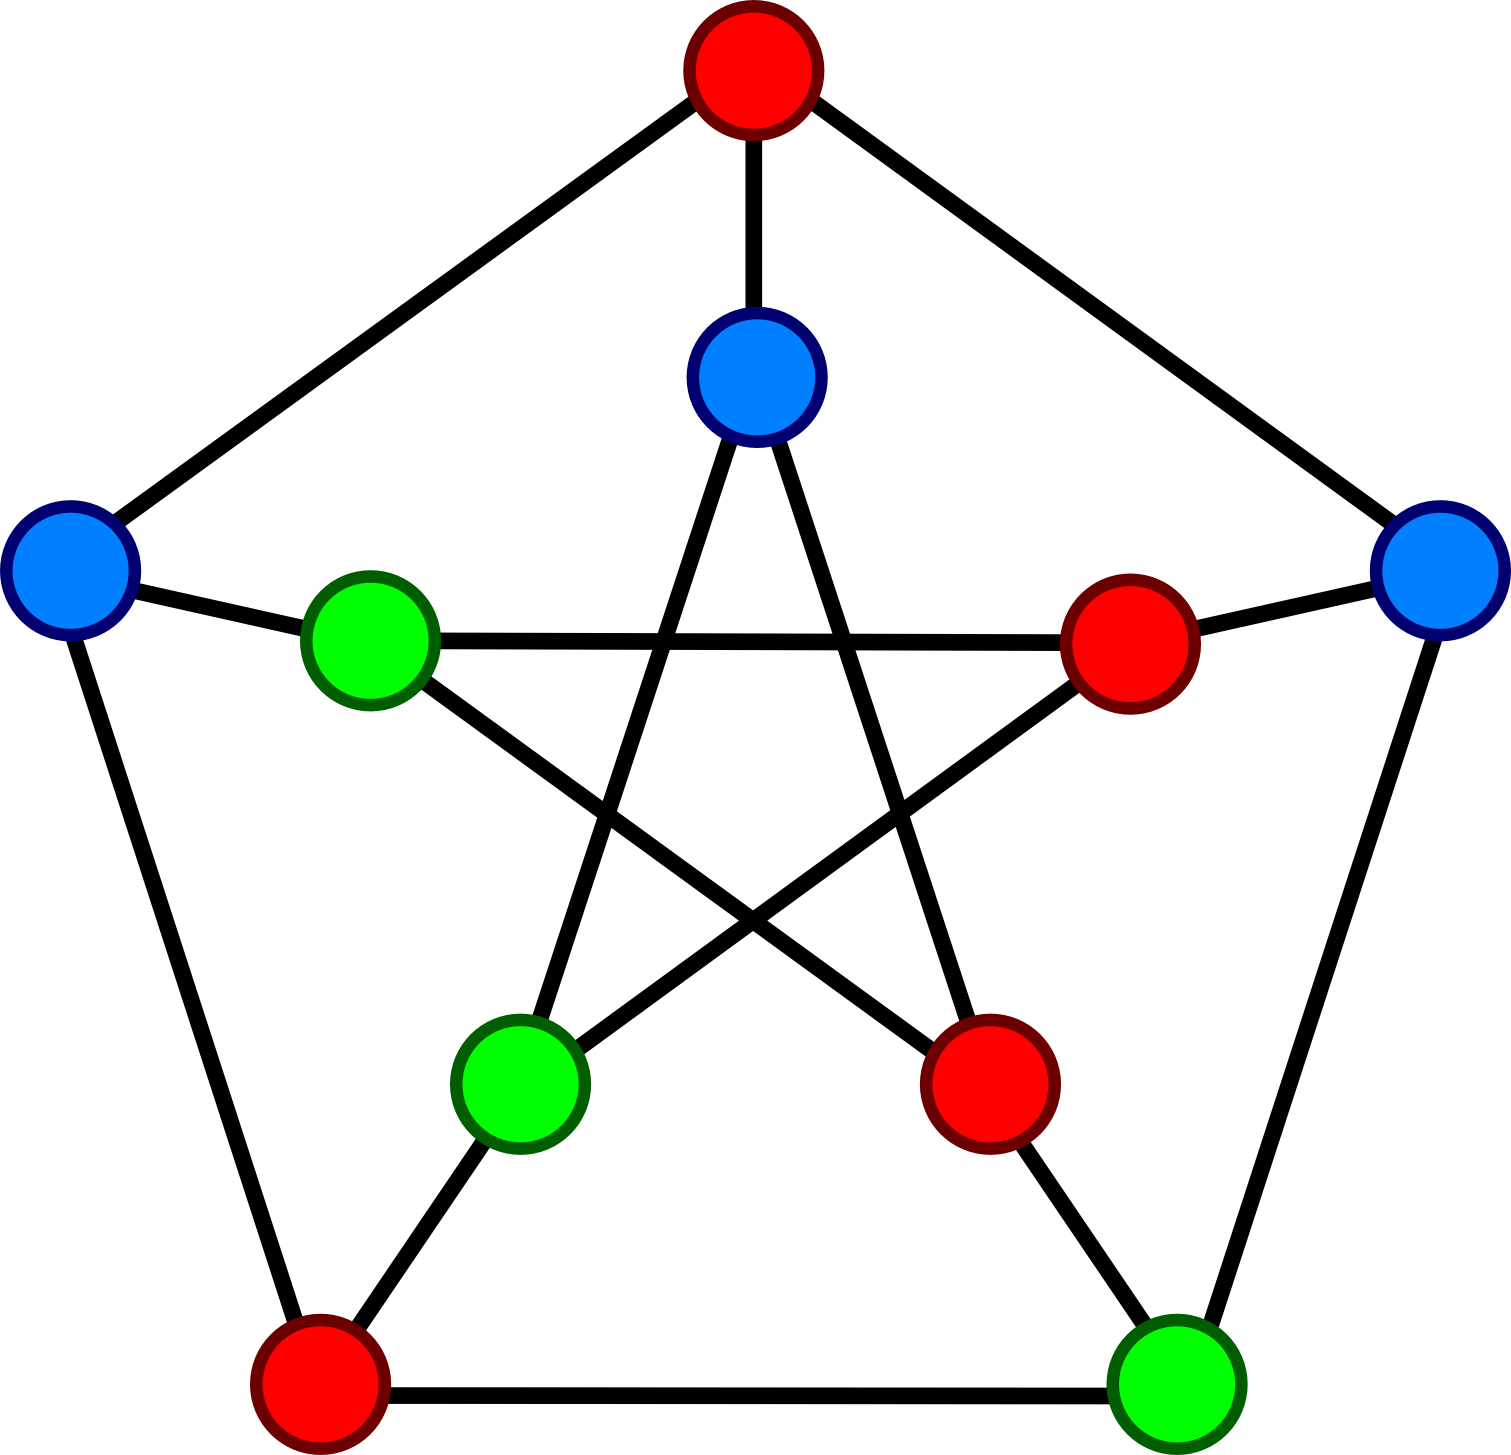
\includegraphics[width=2.5cm]{images/graph3}}%
%
\raisebox{5mm}{%
\hspace{7mm}%
\uncover<3->{\begin{minipage}[b]{6cm}
Darstellung von Farben mit Atomen:
\begin{itemize}
\item $\ppred{i}$ bedeutet "`Knoten $i$ ist rot"'
\item $\pgreen{i}$ bedeutet "`Knoten $i$ ist grün"'
\item $\pblue{i}$ bedeutet "`Knoten $i$ ist blau"'
\end{itemize}
\end{minipage}}}
\bigskip

\uncover<4->{
Färbe-Bedingungen für Knoten:
$(\ppred{1}\wedge\neg\pgreen{1}\wedge\neg\pblue{1})\vee
(\neg\ppred{1}\wedge\pgreen{1}\wedge\neg\pblue{1})\vee
(\neg\ppred{1}\wedge\neg\pgreen{1}\wedge\pblue{1})$
\\\mbox{}\hfill(usw. für alle Knoten)
% $(\ppred{10}\wedge\neg\pgreen{10}\wedge\neg\pblue{10})\vee
% (\neg\ppred{10}\wedge\pgreen{10}\wedge\neg\pblue{10})\vee
% (\neg\ppred{10}\wedge\neg\pgreen{10}\wedge\pblue{10})$\\
}

\bigskip
\uncover<4->{
Färbe-Bedingungen für Kanten:

$\neg(\ppred{1}\wedge\ppred{2})\wedge\neg(\pgreen{1}\wedge\pgreen{2})\wedge\neg(\pblue{1}\wedge\pblue{2})$
\mbox{}\hfill(usw. für alle Kanten)
}
\uncover<5->{
\begin{center}
\alert{Erfüllende Wertzuweisung $\Leftrightarrow$ zulässige Färbung}
\end{center}
}

\end{frame}

\begin{frame}\frametitle{Polynomielle Reduktionen}

\defbox{Eine Funktion $f:\Sigma^*\to\Sigma^*$ ist \redalert{polynomiell berechenbar} wenn es eine
polynomiell-zeitbeschränkte TM gibt, die bei einer Eingabe $w$ die Ausgabe $f(w)$ auf das Band schreibt
und anschließend anhält.
}\bigskip

\defbox{Eine polynomiell berechenbare Funktion $f:\Sigma^*\to\Sigma^*$ ist eine \redalert{polynomielle Reduktion} von einer
Sprache $\Slang{L}$ auf eine Sprache $\Slang{G}$, wenn für alle Wörter $w\in\Slang{L}$ gilt:\\[1ex]
%
\narrowcentering{$w\in\Slang{L}\quad$ genau dann wenn $\quad f(w)\in\Slang{G}$}
}\bigskip\pause

\examplebox{Beispiel: Die soeben skizzierte Funktion von Graphen auf logische Formeln ist eine polynomielle Reduktion
des Drei-Farben-Problems auf \Slang{SAT}.}

\examplebox{Beispiel: Wir haben das Äquivalenzproblem endlicher Automaten in Vorlesung~10 polynomiell auf das Inklusionsproblem reduziert.}

\end{frame}

\begin{frame}[t]\frametitle{Die Struktur von NP}
Idee: polynomielle Reduzierbarikeit definiert eine Art Ordnung auf Problemen

\vspace{1cm}
\begin{center}
\only<1>{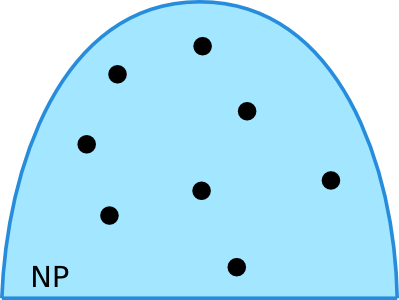
\includegraphics[scale=1.5]{images/np1}}%
\only<2>{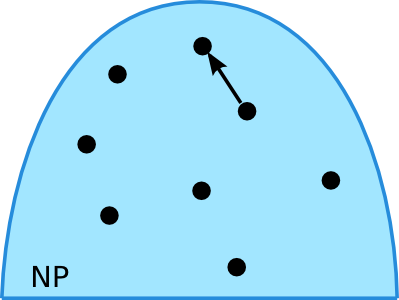
\includegraphics[scale=1.5]{images/np2}}%
\only<3>{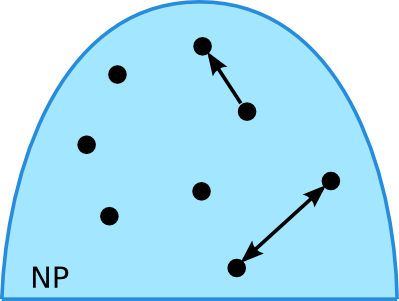
\includegraphics[scale=1.5]{images/np3}}%
\only<4>{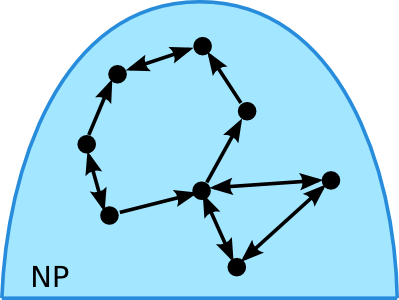
\includegraphics[scale=1.5]{images/np4}}%
\only<5>{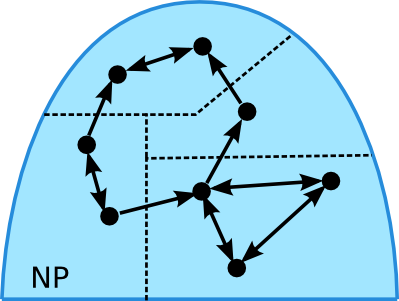
\includegraphics[scale=1.5]{images/np5}}
\end{center}

\end{frame}


\begin{frame}\frametitle{Das schwerste Problem in NP?}

\bigskip
~\hfill%
\begin{minipage}{1.5cm}
\includegraphics[height=1.4cm]{images/cook}\\\scalebox{0.8}{Stephen Cook}\end{minipage}\hfill
\begin{minipage}{1.5cm}
\includegraphics[height=1.4cm]{images/levin}\\\scalebox{0.8}{Leonid Levin}\end{minipage}\hfill
\begin{minipage}{1.5cm}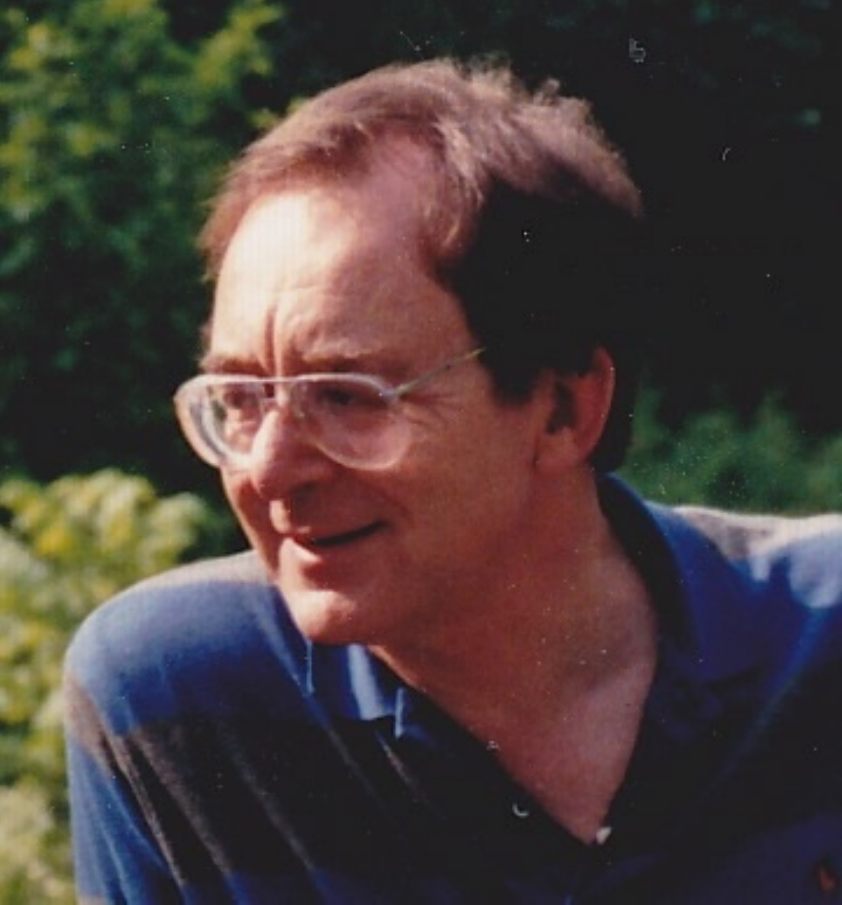
\includegraphics[height=1.4cm]{images/karp}\\\scalebox{0.8}{Richard Karp}\end{minipage}\hfill~
\bigskip

\theobox{Satz von Cook [1971] \& Levin [1973]:
Alle Probleme in \Scomplclass{NP} können polynomiell auf \Slang{SAT} reduziert werden.}\pause

\begin{itemize}
\item Wer \Slang{SAT} polynomiell löst, der hat alle Probleme in \Scomplclass{NP} polynomiell gelöst\pause
\item Es gibt in \Scomplclass{NP} eine maximale Klasse, die ein praktisch interessantes Problem enthält\pause
\item Karp findet kurz darauf 21 weitere solcher Probleme (1972)
\item Seitdem wurden tausende weitere entdeckt \ldots
\end{itemize}
% \pause
\bigskip
% $\leadsto$ Die Klasse der "`schwersten"' Probleme in NP ist praktisch interessant


\end{frame}

\begin{frame}\frametitle{\Scomplclass{NP}-Härte und \Scomplclass{NP}-Vollständigkeit}

\defbox{Eine Sprache ist
\begin{itemize}
\item \redalert{\Scomplclass{NP}-hart,} wenn jede Sprache in \Scomplclass{NP} polynomiell darauf reduzierbar ist
\item \redalert{\Scomplclass{NP}-vollständig,} wenn sie \Scomplclass{NP}-hart ist und in \Scomplclass{NP} liegt
\end{itemize}}\medskip\pause

\examplebox{Beispiel: \Slang{SAT} ist \Scomplclass{NP}-vollständig (Cook \& Levin).}

\examplebox{Beispiel: \Slang{PRIMES} ist in \Scomplclass{NP}, aber \alert{vermutlich} nicht \Scomplclass{NP}-hart. Gleiches gilt für viele Probleme in \Scomplclass{P} (bei einigen ist dagegen sicher, dass sie nicht \Scomplclass{NP}-hart sind).}

\examplebox{Beispiel: Das Halteproblem ist \Scomplclass{NP}-hart aber sicher nicht in \Scomplclass{NP}. Gleiches gilt für jedes unentscheidbare Problem.}


\end{frame}

\begin{frame}\frametitle{Beispiele}

\examplebox{Beispiel: Das Drei-Farben-Problem ist \Scomplclass{NP}-vollständig.}

\examplebox{Beispiel: Verallgemeinertes Sudoku ($n$ Zahlen in einem $n^2\times n^2$-Feld mit $n\times n$-Unterfeldern) ist \Scomplclass{NP}-vollständig. Das Entscheidungsproblem dabei ist, ob das gegebene, teilweise gefüllte Feld eine Lösung zulässt. Gleiches gilt für Verallgemeinerungen vieler anderer Solitärspiele (z.B. Minesweeper).}

\examplebox{Beispiel: Das Wortproblem für Typ-1-Sprachen (gegeben als Grammatik) ist \Scomplclass{NP}-hart aber \alert{vermutlich} nicht in \Scomplclass{NP}. Gleiches gilt für das Halteproblem von LBAs.}

\examplebox{Beispiel: Das Problem des Handelsreisenden ist \Scomplclass{NP}-vollständig. Es besteht darin, in einem
Graph mit bewerteten Kanten einen Pfad durch alle Knoten zu finden, so dass die Summe der Kantenwerte unter einem
gegebenen Maximum liegt.}

\end{frame}

\begin{frame}\frametitle{Wie findet man \Scomplclass{NP}-harte Probleme?}

Schwer ist, worauf sich schwere Dinge leicht zurückführen lassen:

\theobox{Satz: Wenn $\Slang{L}$ \Scomplclass{NP}-hart ist und polynomiell auf $\Slang{G}$
reduziert werden kann, dann ist $\Slang{G}$ auch \Scomplclass{NP}-hart.}

\emph{Beweis:} Folgt direkt aus der Definition, da die Komposition von zwei polynomiellen Reduktionen ebenfalls eine
polynomielle Reduktion ist.\qed
\bigskip\pause

\emph{Technik zum Beweis von \Scomplclass{NP}-Härte:}
\begin{itemize}
\item Suche ein bekanntes \Scomplclass{NP}-hartes Problem, welches dem untersuchten Problem möglichst ähnlich ist.
\item Gib eine polynomielle Reduktion an und zeige, dass sie korrekt ist.
\end{itemize}
\begin{enumerate}[$\leadsto$]
\item Oft nicht schwer, wenn man bereits viele \Scomplclass{NP}-harte Probleme kennt -- aber wo fängt man an?
\end{enumerate}

\end{frame}

\begin{frame}\frametitle{Das erste \Scomplclass{NP}-vollständige Problem}

Ein Problem ist per Definition \Scomplclass{NP}-vollständig:\\[1ex]

\defbox{Das \redalert{Wortpoblem für polynomiell-zeitbeschränkte nichtdeterministische Turingmaschinen}
besteht darin zu entscheiden, ob ein gegebenes Wort $w$ von einer gegebenen polynomiell-zeitbeschränkten NTM
akzeptiert wird.}

Offenbar kann jedes Problem in \Scomplclass{NP} darauf reduziert werden.
\bigskip

Für den Satz von Cook \& Levin zeigt man die \Scomplclass{NP}-Vollständigkeit von \Slang{SAT} durch Reduktion auf dieses
Urproblem.

\end{frame}

\begin{frame}\frametitle{Cook/Levin: Beweisskizze (1)}

\alert{Wie stellen wir TM-Berechnungen in aussagenlogisch dar?}
\bigskip

\emph{Idee:}
\begin{itemize}
\item Eine Instanz des Wortproblems ist eine polynomiell-zeitbeschränkte NTM \Smach{M} und ein Eingabewort
\item Die Zeitbeschränkung für \Smach{M} kann durch ein konkretes Polynom $p$ angegeben werden
\item Wir kennen also die maximale Zahl an Schritten $p(|w|)$ für diese Berechnung
\end{itemize}
\begin{enumerate}[$\leadsto$]
\item Ein Lauf ist eine Folge von maximal $p(|w|)$ Konfigurationen, die jeweils maximal $p(|w|)$ Speicherstellen verwenden
\end{enumerate}
\bigskip

\emph{Ansatz:} Kodiere \Smach{M} und $w$ so in Logik, dass die möglichen Läufe genau den erfüllenden Wertzuweisungen entsprechen

\end{frame}

\begin{frame}\frametitle{Cook/Levin: Beweisskizze (2)}


% Illustration eines Laufs in $p(|w|)$ Schritten:

\begin{tikzpicture}[
	scale=0.50,
	decoration=penciline, decorate
]
% \path[use as bounding box] (-3.2,0) rectangle (3.5,-5); % add "draw" to see it
% \draw[help lines] (0,0) grid (5,5);
\pgfmathsetseed{5712}

\draw [thick, darkblue,decorate,decoration={brace,amplitude=3pt},xshift=0.4pt,yshift=-0.7mm](-1,0.6) -- (13,0.6) node[black,midway,yshift=0.36cm] {\alert{$p(|w|)$ Speicherstellen}};

\draw [thick, darkblue,decorate,decoration={brace,mirror,amplitude=3pt},xshift=0.4pt,yshift=-0.7mm](-1.5,0) -- (-1.5,-7.5) node[black,midway,xshift=-0.36cm] {\rotatebox{90}{\alert{$p(|w|)$ Berechnungsschritte}}};

\draw[decorate,line width=0.3mm] (-1,0) -- (10.5,0);
\draw[decorate,line width=0.3mm] (-1,-1) -- (10.5,-1);
\node [circle,draw=none,inner sep=1pt] at (11.1,0) {$\cdots$};
\node [circle,draw=none,inner sep=1pt] at (11.1,-1) {$\cdots$};
\draw[decorate,line width=0.3mm] (11.5,0) -- (13,0);
\draw[decorate,line width=0.3mm] (11.5,-1) -- (13,-1);

\foreach \x in {0,...,10} {
	\draw[decorate,line width=0.3mm] (\x-1,0) -- (\x-1,-0.9);
	\node [circle,draw=none,inner sep=1pt] at (\x-0.5,-0.5) {\ifthenelse{\x<5}{\ifthenelse{\x<3}{\Sterm{a}}{\Sterm{b}}}{\ifthenelse{\x=5 \OR \x=7 \OR \x=8}{\Sterm{c}}{\ifthenelse{\x=10}{$\blank$}{\Sterm{d}}}}};
}
\draw[decorate,line width=0.3mm] (10,0) -- (10,-0.9);
\draw[decorate,line width=0.3mm] (12,0) -- (12,-0.9);
\node [circle,draw=none,inner sep=1pt] at (12.5,-0.5) {$\blank$};
\draw[decorate,line width=0.3mm] (13,0) -- (13,-0.9);

\draw[fill=none,line width=0.4mm,darkblue,->] (-0.5,-1.5) -> (-0.5,-1.1);
\node [circle,draw=none,inner sep=1pt] at (-0.5,-1.8) {$q_0$};


\draw[decorate,line width=0.3mm] (-1,-2.5) -- (10.5,-2.5);
\draw[decorate,line width=0.3mm] (-1,-3.5) -- (10.5,-3.5);
\node [circle,draw=none,inner sep=1pt] at (11.1,-2.5) {$\cdots$};
\node [circle,draw=none,inner sep=1pt] at (11.1,-3.5) {$\cdots$};
\draw[decorate,line width=0.3mm] (11.5,-2.5) -- (13,-2.5);
\draw[decorate,line width=0.3mm] (11.5,-3.5) -- (13,-3.5);

\foreach \x in {0,...,10} {
	\draw[decorate,line width=0.3mm] (\x-1,-2.5) -- (\x-1,-3.4);
	\node [circle,draw=none,inner sep=1pt] at (\x-0.5,-3.0) {\ifthenelse{\x=0}{\Snterm{A}}{\ifthenelse{\x<5}{\ifthenelse{\x<3}{\Sterm{a}}{\Sterm{b}}}{\ifthenelse{\x=5 \OR \x=7 \OR \x=8}{\Sterm{c}}{\ifthenelse{\x=10}{$\blank$}{\Sterm{d}}}}}};
}
\draw[decorate,line width=0.3mm] (10,-2.5) -- (10,-3.4);
\draw[decorate,line width=0.3mm] (12,-2.5) -- (12,-3.4);
\node [circle,draw=none,inner sep=1pt] at (12.5,-3) {$\blank$};
\draw[decorate,line width=0.3mm] (13,-2.5) -- (13,-3.4);

\draw[fill=none,line width=0.4mm,darkblue,->] (0.5,-4.0) -> (0.5,-3.6);
\node [circle,draw=none,inner sep=1pt] at (0.5,-4.3) {$q_1$};

\node [circle,draw=none,inner sep=1pt] at (-0.5,-5.2) {$\vdots$};
\node [circle,draw=none,inner sep=1pt] at (9.5,-5.2) {$\vdots$};
\node [circle,draw=none,inner sep=1pt] at (12.5,-5.2) {$\vdots$};

\draw[decorate,line width=0.3mm] (-1,-6.5) -- (10.5,-6.5);
\draw[decorate,line width=0.3mm] (-1,-7.5) -- (10.5,-7.5);
\node [circle,draw=none,inner sep=1pt] at (11.1,-6.5) {$\cdots$};
\node [circle,draw=none,inner sep=1pt] at (11.1,-7.5) {$\cdots$};
\draw[decorate,line width=0.3mm] (11.5,-6.5) -- (13,-6.5);
\draw[decorate,line width=0.3mm] (11.5,-7.5) -- (13,-7.5);

\foreach \x in {0,...,10} {
	\draw[decorate,line width=0.3mm] (\x-1,-6.5) -- (\x-1,-7.4);
	\node [circle,draw=none,inner sep=1pt] at (\x-0.5,-7.0) {\ifthenelse{\x=2}{\Snterm{B}}{\ifthenelse{\x<5}{\ifthenelse{\x<3}{\Snterm{A}}{\Sterm{a}}}{\ifthenelse{\x=5 \OR \x=7 \OR \x=8}{\Snterm{C}}{\ifthenelse{\x=10}{\Snterm{A}}{\Sterm{b}}}}}};
}
\draw[decorate,line width=0.3mm] (10,-6.5) -- (10,-7.4);
\draw[decorate,line width=0.3mm] (12,-6.5) -- (12,-7.4);
\node [circle,draw=none,inner sep=1pt] at (12.5,-7) {\Snterm{B}};
\draw[decorate,line width=0.3mm] (13,-6.5) -- (13,-7.4);

\draw[fill=none,line width=0.4mm,darkblue,->] (5.5,-8.0) -> (5.5,-7.6);
\node [circle,draw=none,inner sep=1pt] at (5.5,-8.4) {$q_f$};

\end{tikzpicture}

Wir können diesen Lauf mit aussagenlogischen Atomen kodieren:
\begin{itemize}
\item $Q_{q,s}$: "`TM ist in Schritt $s$ in Zustand $q$"'
% 
% Für jede Position $i\in\{1,\ldots,p(|w|)\}$, jeden Schritt $s\in\{1,\ldots,p(|w|)\}$
\item $P_{i,s}$: "`TM-Kopf ist in Schritt $s$ an Position $i$"'
\item $S_{a,i,s}$: "`Das Band enthält in Schritt $s$ Zeichen $a$ an Position $i$"'
\end{itemize}

\end{frame}

\begin{frame}\frametitle{Cook/Levin: Beweisskizze (3)}

Wir können diesen Lauf mit aussagenlogischen Atomen kodieren:
\begin{itemize}
\item $Q_{q,s}$: "`TM ist in Schritt $s$ in Zustand $q$"'
% 
% Für jede Position $i\in\{1,\ldots,p(|w|)\}$, jeden Schritt $s\in\{1,\ldots,p(|w|)\}$
\item $P_{i,s}$: "`TM-Kopf ist in Schritt $s$ an Position $i$"'
\item $S_{a,i,s}$: "`Das Band enthält in Schritt $s$ Zeichen $a$ an Position $i$"'
\end{itemize}
$\leadsto$ Nur polynomiell viele Atome nötig
\bigskip

Mithilfe von Formeln kann man alle Bedingungen ausdrücken, die für einen korrekten Lauf der NTM gelten müssen.

% , z.B.
% dass  zu jedem Zeitpunkt nur ein Zustand gilt ($Q_{q,s}\to\neg Q_{q',s}$ für alle $s\in\{1,\ldots,p(|w|)\}$ und Zustände $q\neq q'$).
\medskip

\examplebox{
Die Übergangsrelation wird z.B. mit Formel der folgenden Form kodiert:
\[(Q_{q,s}\wedge P_{i,s}\wedge S_{a,i,s})\to\bigvee_{\substack{\tuple{q',b,D}\in\delta(q,a)\\ i'=D(i)}} (S_{b,i,s+1}\wedge Q_{q',s+1}\wedge P_{i',s+1})\]
(für alle $s\in\{1,\ldots,p(|w|)\}$ und Positionen $i\in\{1,\ldots,p(|w|)\}$).}


\end{frame}

\begin{frame}\frametitle{Deterministisch vs. Nichtdeterministisch}

	Wir haben bereits bemerkt, dass \Scomplclass{P} ${}\subseteq{}$ \Scomplclass{NP} gilt, da DTMs spezielle NTMs sind.
	\medskip

  \alert{Bis heute ist nicht bekannt, ob die Umkehrung dieser Inklusion gilt oder nicht.}
  \begin{itemize}
  \item Intuitiv gefragt: "`Wenn es einfach ist, eine mögliche Lösung für ein Problem zu prüfen, ist es dann auch einfach, eine zu finden?"'
  \item Übertrieben: "`Can creativity be automated?"' (Wigderson, \ghost{2006)}
  \item Seit über 40 Jahren ungelöst
  \item Eines der größten offenen Probleme der Informatik und Mathematik unserer Zeit
  \item 1.000.000 USD Preisgeld für die Lösung\\("`Millenium Problem"')
  \end{itemize}
   
\end{frame}

%%%%%%%%%%%%%%%%%%%%%%%%%%%%%%%%%%%%%%%%%%%%%%%%%%%%%%%%%%%%%%%%%%%%%
% \begin{frame}\frametitle{Status of \PTime vs. \NP}
% %   So what is the state of this question?
% 
%   \begin{itemize}
%   \item It is often said: \alert{``Most experts think \PTime ${}\neq{}$ \NP''}
% 	\begin{itemize}
% 	\item Main argument: ``If $\NP = \PTime$, someone ought to have found some polynomial algorithm by now.''
% 	\item ``This is, in my opinion, a very weak argument. The space of algorithms is very large and we are only at the beginning of its exploration.'' (Moshe Vardi, 2002)
% 	\end{itemize}
%   \item Results of a poll among 100 experts [Gasarch 2002]:
% 	\begin{itemize}
% 	\item $\PTime \neq \NP$: 61
% 	\item $\PTime = \NP$: 9
% 	\item No comment: 22
% 	\item Other: independent (4), not independent (3), it depends (1)
% 	\end{itemize}
%   \item Over 100 ``proofs'' show $\PTime = \NP$ to be true/false/both/neither: \url{https://www.win.tue.nl/~gwoegi/P-versus-NP.htm}
%   \item Many solutions conceivable, e.g., $\PTime = \NP$ could be shown with a non-constructive proof
%   \end{itemize}
%    
% \end{frame}

%%%%%%%%%%%%%%%%%%%%%%%%%%%%%%%%%%%%%%%%%%%%%%%%%%%%%%%%%%%%%%%%%%%%%
\begin{frame}\frametitle{Status von \Scomplclass{P} vs. \Scomplclass{NP}}
%   So what is the state of this question?

  Viele Menschen glauben \Scomplclass{P} ${}\neq{}$ \Scomplclass{NP}
	\begin{itemize}
	\item Hauptargument: "`Wenn $\Scomplclass{NP} = \Scomplclass{P}$ wäre, dann müsste jemand inzwischen einen polynomiellen Algorithmus für ein \Scomplclass{NP}-vollständiges Problem gefunden haben."'
	\item ``This is, in my opinion, a very weak argument. The space of algorithms is very large and we are only at the beginning of its exploration.'' (Moshe Vardi, 2002)
	\item Ein weiterer Grund für die verbreitete Meinung: Menschen finden es schwer, \Scomplclass{NP}-Probleme zu lösen und können sich schwer vorstellen, wie man sie vereinfachen sollte
	-- eventuell ``human chauvinistic bravado'' (Zeilenberger, 2006)
	\item Es gibt noch bessere Argumente, aber keines mehr als eine Intuition
	\end{itemize}
\end{frame}

%%%%%%%%%%%%%%%%%%%%%%%%%%%%%%%%%%%%%%%%%%%%%%%%%%%%%%%%%%%%%%%%%%%%%
\begin{frame}\frametitle{Status von \Scomplclass{P} vs. \Scomplclass{NP} (2)}
%   So what is the state of this question?

  Verschiedene Ergebnisse sind denkbar:\pause
  \begin{itemize}
	\item $\Scomplclass{P} =  \Scomplclass{NP}$ könnte durch einen nicht-konstruktiven Beweis gezeigt werden\pause
	\item Die Antwort könnte unabhängig von den Standardaxiomen der Mathematik (ZFC) sein\pause
	\item Selbst wenn $\Scomplclass{P} \neq \Scomplclass{NP}$ gilt, ist weiterhin unklar, ob $\Scomplclass{NP}$-harte Problem wirklich exponentielle Zeit benötigen -- es gibt viele andere super-polynomielle Funktionen \ldots\pause
	\item Das Problem könnte für immer ungelöst bleiben\pause
  \end{itemize}\bigskip
  
  Über 100 "`Beweise"' zeigen, dass $\Scomplclass{P} = \Scomplclass{NP}$ wahr/falsch/beides/keines der beiden ist: \url{https://www.win.tue.nl/~gwoegi/P-versus-NP.htm}
   
\end{frame}

%%%%%%%%%%%%%%%%%%%%%%%%%%%%%%%%%%%%%%%%%%%%%%%%%%%%%%%%%%%%%%%%%%%%%
% \begin{frame}\frametitle{Status von \Scomplclass{P} vs. \Scomplclass{NP} (3)}
% %   So what is the state of this question?
% 
%   Aktuelle Meinung in der Forschung:
%   \begin{itemize}
%   \item Ergebnisse einer Umfrage unter 152 Experten [Gasarch 2012]:
% 	\begin{itemize}
% 	\item $\Scomplclass{P} \neq \Scomplclass{NP}$: 126 (83\%)
% 	\item $\Scomplclass{P} = \Scomplclass{NP}$: 12 (9\%)
% 	\item Weiß nicht/ist mir egal: 7 (4\%)
% 	\item Unabhängig von ZFC: 5 (3\%)
% 	\item "`I don't \emph{want} it to be equal."': 1 (0.6\%)
% 	\end{itemize}
%   \item Experten haben sich auch schon früher geirrt
%   \item Über 100 "`Beweise"' zeigen, dass $\Scomplclass{P} = \Scomplclass{NP}$ wahr/falsch/beides/keines der beiden ist: \url{https://www.win.tue.nl/~gwoegi/P-versus-NP.htm}
% %   \item Research journals have policies to limit the number of ``proofs'' submitted per year
%   \end{itemize}
%    
% \end{frame}

\begin{frame}\frametitle{\Scomplclass{P}-Härte}

Man kann Härte und Vollständigkeit auch für andere Klassen definieren. Bei schwächeren Klassen
muss man allerdings sicherstellen, dass die Reduktion selbst nicht schon so viele Ressourcen benötigt wie
die Lösung des Problems!

\defbox{Eine Sprache ist \Scomplclass{P}-hart wenn jede Sprache in \Scomplclass{P} mit logarithmischem Speicherbedarf
darauf reduzierbar ist. Sie ist \Scomplclass{P}-vollständig, wenn sie zudem in \Scomplclass{P} liegt.}\pause

\begin{itemize}
\item \Scomplclass{P}-vollständige Probleme sind die schwersten polynomiell lösbaren Probleme.
\item Sie gelten als inhärent seriell, d.h. als nicht gut parallelisierbar (bisher nicht bewiesen).
\end{itemize}\pause

\examplebox{Beispiel: Die Erfüllbarkeit von aussagenlogischen Horn-Formeln (\Slang{HornSAT}) ist ein \Scomplclass{P}-vollständiges Problem.}

\end{frame}


\begin{frame}\frametitle{Zusammenfassung und Ausblick}

\Scomplclass{NP} ist die Klasse der \redalert{nachweis-polynomiellen Probleme}.
\bigskip

\redalert{\Scomplclass{NP}-vollständige} Probleme sind die schwersten Probleme in \Scomplclass{NP}: Wenn man eines davon effizient löst, dann kann alle Probleme in \Scomplclass{NP} effizient lösen.
\bigskip

\redalert{\Slang{SAT} ist $\Scomplclass{NP}$-vollständig} und \redalert{\Slang{HornSAT} ist $\Scomplclass{P}$-vollständig}.
\bigskip

\anybox{yellow}{
Offene Fragen:
\begin{itemize}
\item Wie genau stehen die Komplexitätsklassen in Beziehung? Insbesondere: $\Scomplclass{P}\neq \Scomplclass{NP}$?
\item Haben Sie noch inhaltliche Fragen? ($\leadsto$ Mailingliste!)
\item Haben Sie sich ausreichend auf die Prüfung vorbereitet?
\end{itemize}
}

\end{frame}


\end{document}